%! Author = gcpease
%! Date = 4/20/21

% Preamble
\documentclass[border=5mm]{article}
\usepackage{pgfplots}
\usetikzlibrary{arrows.meta}

% Packages
\usepackage{amsmath}
\usepackage[utf8]{inputenc}
\usepackage[a4paper, total={8in, 10in}]{geometry}
\usepackage{paracol}
\usepackage{titling}
\newcommand{\linespace}{\vspace{1cm}}
\setlength{\columnseprule}{0.2pt}
\usepackage{tikz}

% Document
\begin{document}
    \centerline {02 - Graphing}
    \centerline {Remember that graphs are in the form of $y=Mx+b$}
    \centerline {Where $M$ = $\frac{rise}{run}$, and $b$ is a constant.}
    \begin{paracol}{2}
        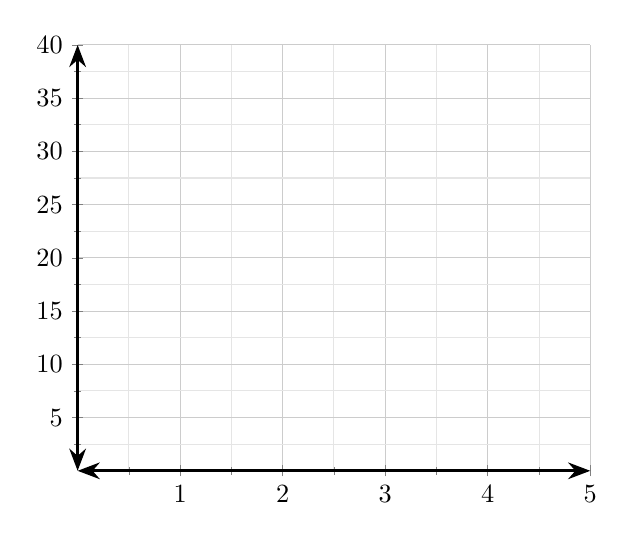
\begin{tikzpicture}[scale=0.95]
            \begin{axis}[
            axis lines=middle,
            axis line style={Stealth-Stealth,very thick},
            xmin=0,xmax=5,ymin=0,ymax=40,
            minor tick num=1,
            xtick distance=1,
            ytick distance=5,
            grid=both,
            major grid style={thin,black!20},
            minor grid style={thin,black!10}]
            \end{axis}
        \end{tikzpicture}
        \begin{enumerate}
            \item Supposed John walks 8 miles every day.
            \begin{enumerate}
                \item Label the X axis.
                \item Label the Y axis.
                \item Graph how many miles John has walked by day 5.
                \item Label this line as $J$.
            \end{enumerate}
            \item Now suppose that George walks 4 miles a day, but takes a break on day 3 and does not walk.
            \begin{enumerate}
                \item Graph how many miles George walked by day 5.
                \item Label this line as $G$.
            \end{enumerate}
            \item How many less miles has George walked than John?
        \end{enumerate}
        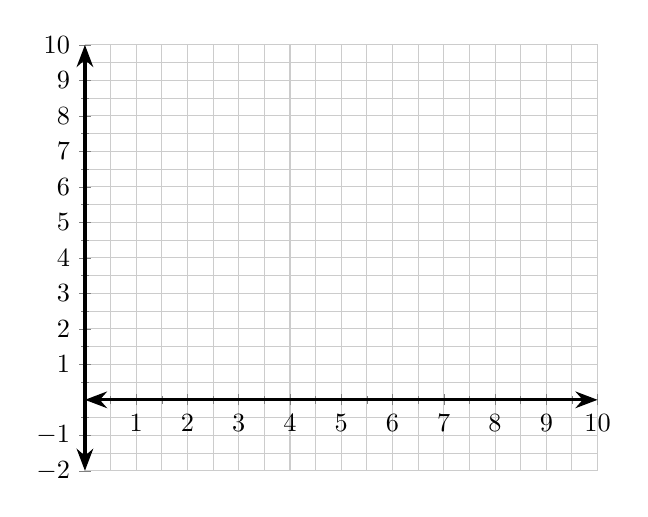
\begin{tikzpicture}[scale=0.95]
            \begin{axis}[
            axis lines=middle,
            axis line style={Stealth-Stealth,very thick},
            xmin=0,xmax=10,ymin=-2,ymax=10,
            minor tick num=1,
            xtick distance=1,
            ytick distance=1,
            grid=both,
            major grid style={thin,black!20},
            minor grid style={thin,black!20}]
            \end{axis}
        \end{tikzpicture}
        \begin{enumerate}
            \setcounter{enumi}{3}
            \item You are driving a car, and you move at $1ft$ per minute.
            \begin{enumerate}
                \item Label the X axis.
                \item Label the Y axis.
                \item You drive forward for 3 minutes. Plot a point at the location you are at.
                \item You now reverse for 4 minutes. Plot a point at the location you are at.
                \item You drive forward for 1 minute. Plot a point at the location you are at.
                \item You remain idle for a minute. Plot a point at the location you are at.
            \end{enumerate}
        \end{enumerate}
        \switchcolumn
        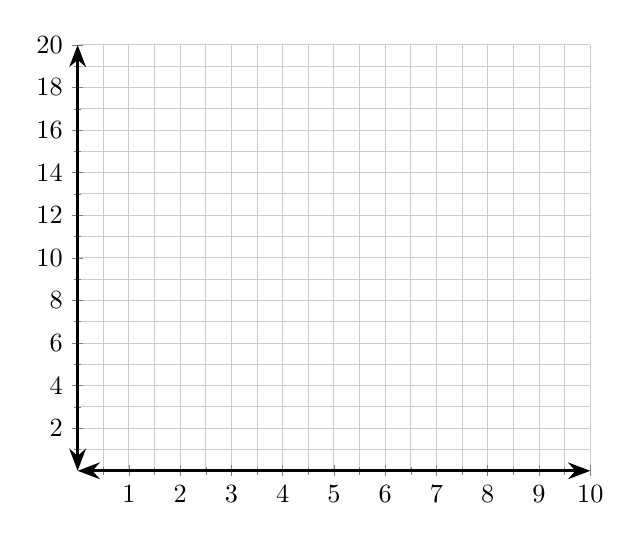
\begin{tikzpicture}[scale=0.95]
            \begin{axis}[
            axis lines=middle,
            axis line style={Stealth-Stealth,very thick},
            xmin=0,xmax=10,ymin=0,ymax=20,
            minor tick num=1,
            xtick distance=1,
            ytick distance=2,
            grid=both,
            major grid style={thin,black!20},
            minor grid style={thin,black!20}]
            \end{axis}
        \end{tikzpicture}
        \begin{enumerate}
            \setcounter{enumi}{4}
            \item   Suppose you fill a container of water at the rate of $2ft$ of water per minute.
            \begin{enumerate}
                \item Label the $X$ axis.
                \item Label the $Y$ axis.
                \item Plot a points of how much water is the container at every minute.
                \item Complete the graph, label it as $T$.
            \end{enumerate}
            \item Suppose that at $6$ minutes your hose breaks, and you can't fill water for another $10$ minutes.
            \begin{enumerate}
                \item Plot a points of how much water is the container at every minute.
                \item Complete the graph, label it as $P$.
            \end{enumerate}
            \item How much more water is in $T$ than $P$?
        \end{enumerate}
        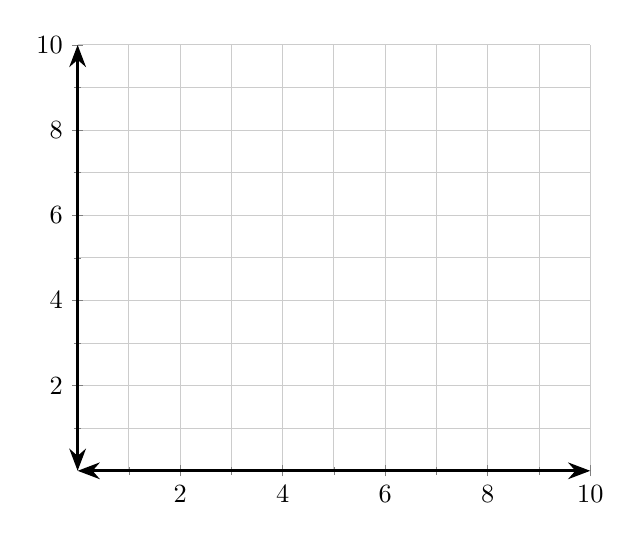
\begin{tikzpicture}[scale=0.95]
            \begin{axis}[
            axis lines=middle,
            axis line style={Stealth-Stealth,very thick},
            xmin=0,xmax=10,ymin=0,ymax=10,
            minor tick num=1,
            xtick distance=2,
            ytick distance=2,
            grid=both,
            major grid style={thin,black!20},
            minor grid style={thin,black!20}]
            \end{axis}
        \end{tikzpicture}
        \begin{enumerate}
            \setcounter{enumi}{7}
            \item Plot the graph $Y=\frac12x+1$ [Hint: Think about rise-over-run]
            \begin{enumerate}
                \item Label the $X$ axis.
                \item Label the $Y$ axis.
                \item Plot all possible values [Hint: For each x coordinate, set x equal to that value in $Y$]
                \item Connect the points, label the line as $A$.
            \end{enumerate}
        \end{enumerate}
    \end{paracol}
\end{document}